La validazione empirica di un'architettura distribuita richiede un'analisi quantitativa volta a isolare le prestazioni dei singoli strati computazionali e di persistenza. Poiché i moderni paradigmi cloud-native disaccoppiano le fasi di ingestione, trasformazione e presentazione delle informazioni, una valutazione olistica risulterebbe imprecisa. Per tale motivo logico, il presente capitolo frammenta l'indagine in tre fasi distinte, progettate per misurare progressivamente l'impatto delle singole scelte implementative. La prima fase definisce la metodologia di collaudo. La seconda fase analizza le prestazioni dei processi asincroni di elaborazione dati. Infine, la terza fase quantifica le latenze dei servizi sincroni e i tempi di approvvigionamento infrastrutturale.

L'ambiente di collaudo consiste in un'infrastruttura di laboratorio progettata per fungere da setting simulato di un ecosistema aziendale operante nel dominio dell'advertising digitale. Per garantire la validità scientifica delle misurazioni senza fare affidamento su generatori di traffico sintetico, l'ambiente isolato si interfaccia direttamente con le piattaforme esterne di produzione. Il sistema elabora parametri e volumi di traffico estratti da un reale caso industriale aziendale, il quale ha fornito le autorizzazioni necessarie per l'interrogazione dei dati.

Questo approccio metodologico garantisce che i volumi di carico, quantificati in circa trenta Gigabyte mensili di dati grezzi, e le latenze di rete registrate riflettano fedelmente la complessità operativa di uno scenario autentico. L'infrastruttura di monitoraggio delega la raccolta dei dati ai componenti nativi del provider cloud, come Amazon CloudWatch e Amazon Athena, generando metriche oggettive sul comportamento del sistema sotto sforzo.

\section{Obiettivi della Valutazione}
L'implementazione dell'architettura software fornisce i componenti tecnici per l'elaborazione dei flussi informativi ad alto volume. Tuttavia, la sola definizione dell'infrastruttura tramite il paradigma Infrastructure as Code governato da Terraform non è sufficiente a dimostrare il superamento dei limiti operativi riscontrati nei sistemi tradizionali. Un'architettura distribuita necessita di una validazione quantitativa per confermare la scalabilità e la stabilità delle prestazioni sotto carico.

\section{Metodologia di Collaudo e Strumenti di Telemetria}
Il collaudo dell'architettura prescinde dall'iniezione di traffico artificiale, adottando una metodologia di analisi osservazionale basata sui carichi di lavoro organici estratti da sistemi in produzione. La validazione empirica aggrega e analizza statisticamente i dati di telemetria raccolti in un arco temporale definito, valutando il comportamento del sistema a regime. L'esclusione di strumenti di stress testing attivi garantisce che le misurazioni riflettano le latenze di rete effettive e i pattern di accesso tipici delle integrazioni tra sistemi distribuiti.

La piattaforma cloud delega la raccolta dei dati a due servizi nativi. Il primo strumento è Amazon CloudWatch, impiegato per il campionamento delle metriche prestazionali a livello di infrastruttura. L'analisi estrae tramite questo servizio i tempi di esecuzione delle funzioni AWS Lambda (metrica \texttt{Duration}), l'allocazione della memoria e il consumo di capacità di lettura e scrittura delle tabelle Amazon DynamoDB. Il servizio provvede inoltre al calcolo automatico dei percentili statistici ($p50$, $p90$, $p99$) relativi alle latenze di integrazione esposte da Amazon API Gateway.

Il secondo strumento di validazione quantitativa risiede nelle metriche di esecuzione di Amazon Athena. Il motore di query traccia il volume di dati scansionati e i millisecondi di elaborazione per ciascuna transazione SQL. L'incrocio di questi valori con la topologia del partizionamento fisico su Amazon S3 fornisce le evidenze necessarie per dimostrare il contenimento della complessità computazionale e il conseguente abbattimento dei costi operativi.

\section{Caso di Studio I: Pipeline ETL Asincrona}
Il primo caso di studio esamina la pipeline ETL incaricata di ingerire la reportistica generata da piattaforme esterne di ad-serving \cite{GoogleAdManager}. L'elaborazione di tali flussi informativi estrae metriche granulari sulle campagne pubblicitarie, fornendo dati aggregati su impressioni, costi e formati. L'architettura applica i pattern definiti nei capitoli precedenti per eseguire l'estrazione periodica di questi dataset complessi. L'obiettivo dell'analisi consiste nel validare la stabilità del runtime Serverless in elaborazioni prolungate e misurare l'efficienza della compressione dei dati.

\subsection{Scenario Operativo e Prestazioni di Estrazione}
Lo scenario operativo impiega regole temporali su Amazon EventBridge, le quali governano l'esecuzione del livello di estrazione isolando le singole transazioni. Come illustrato nella Figura \ref{fig:cloudwatch-extractor}, l'aggregazione delle metriche rileva un regime stabile di circa 140-150 invocazioni giornaliere. Il sistema dimostra la capacità di scalare orizzontalmente, assorbendo picchi di oltre 3.200 invocazioni giornaliere senza registrare degrado prestazionale durante le fasi di ri-computazione dei dati storici.

\begin{figure}[htbp]
\centering
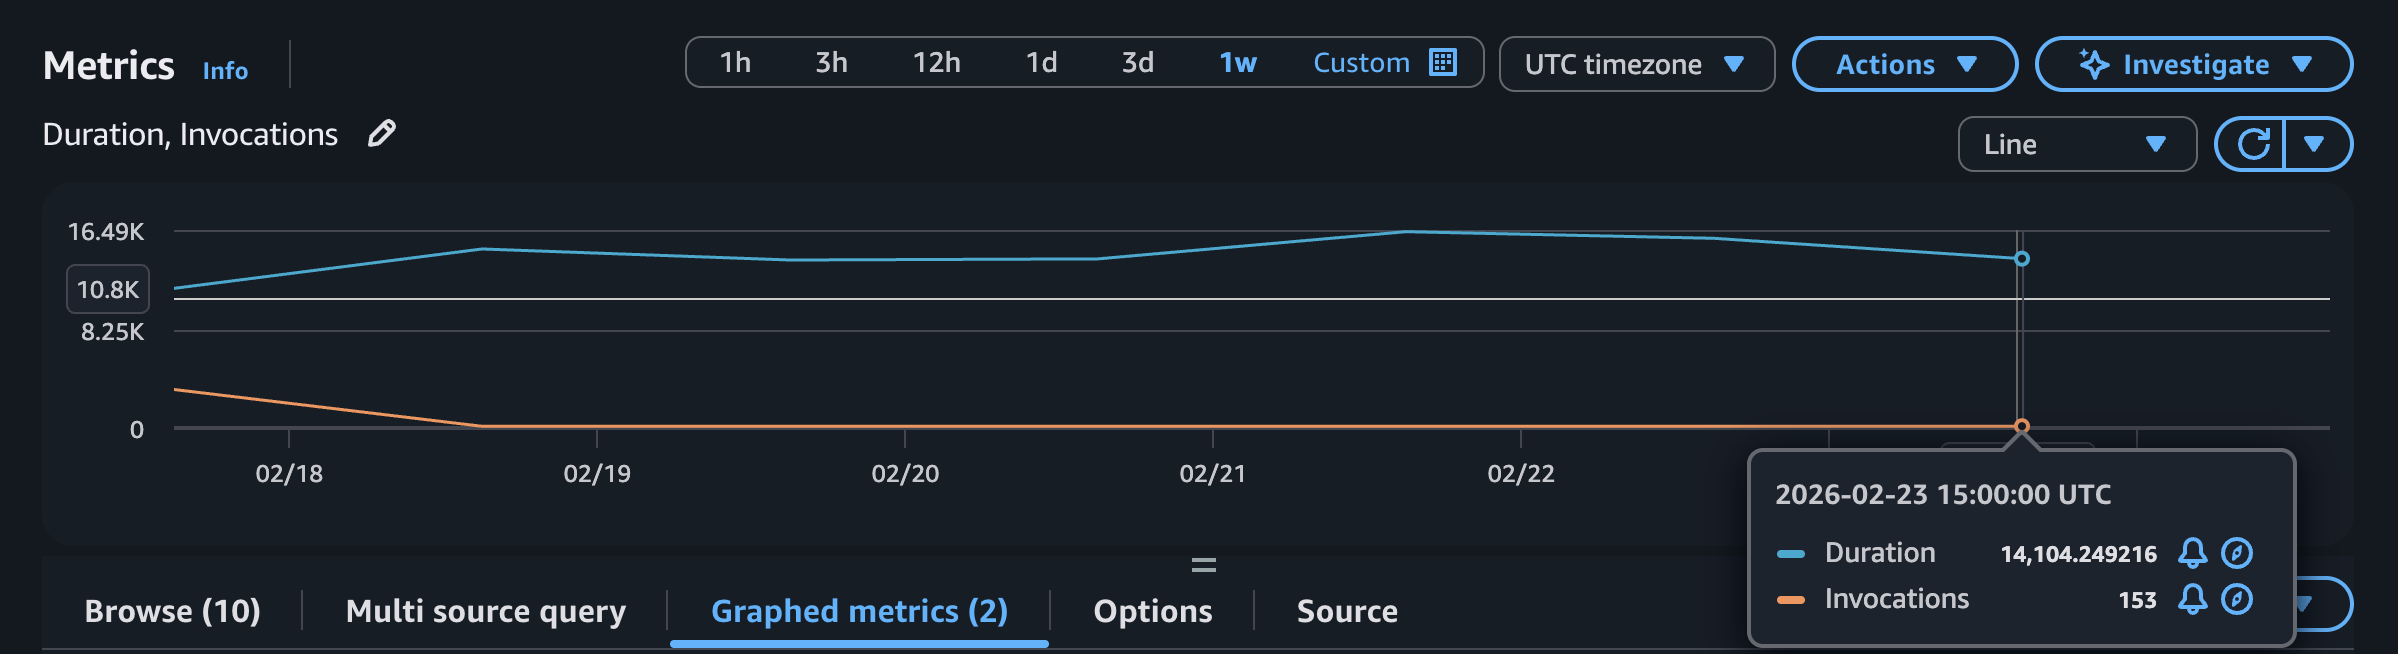
\includegraphics[width=1\textwidth]{images/invocations-durations-extractor.png}
\caption{Grafico CloudWatch illustrante il volume di invocazioni e la metrica Duration del livello Extractor.}
\label{fig:cloudwatch-extractor}
\end{figure}

L'analisi della metrica di durata evidenzia un tempo medio di esecuzione per l'estrazione dati compreso tra $14.000$ e $16.350$ millisecondi per singola invocazione. Questo valore certifica che il componente opera con un margine di tolleranza elevato rispetto al vincolo massimo di 900 secondi imposto dal provider. Il tasso di errore di rete, registrato allo $1,3\%$, giustifica empiricamente l'implementazione della logica di ritentativo applicativo e l'uso delle Dead Letter Queue (DLQ).

\subsection{Efficienza della Trasformazione in Memoria}
La fase di trasformazione, responsabile dell'appiattimento e della sanificazione dei documenti JSON, sfrutta la libreria Polars per l'elaborazione vettoriale in memoria. Le metriche documentano un tempo medio di esecuzione pari a $1.160$ millisecondi, con un tasso di errore dello $0\%$, come indicato nella Figura \ref{fig:transformer-graphic}. Tale efficienza computazionale previene la saturazione della memoria preallocata all'interno dei container.

\begin{figure}[htbp]
\centering
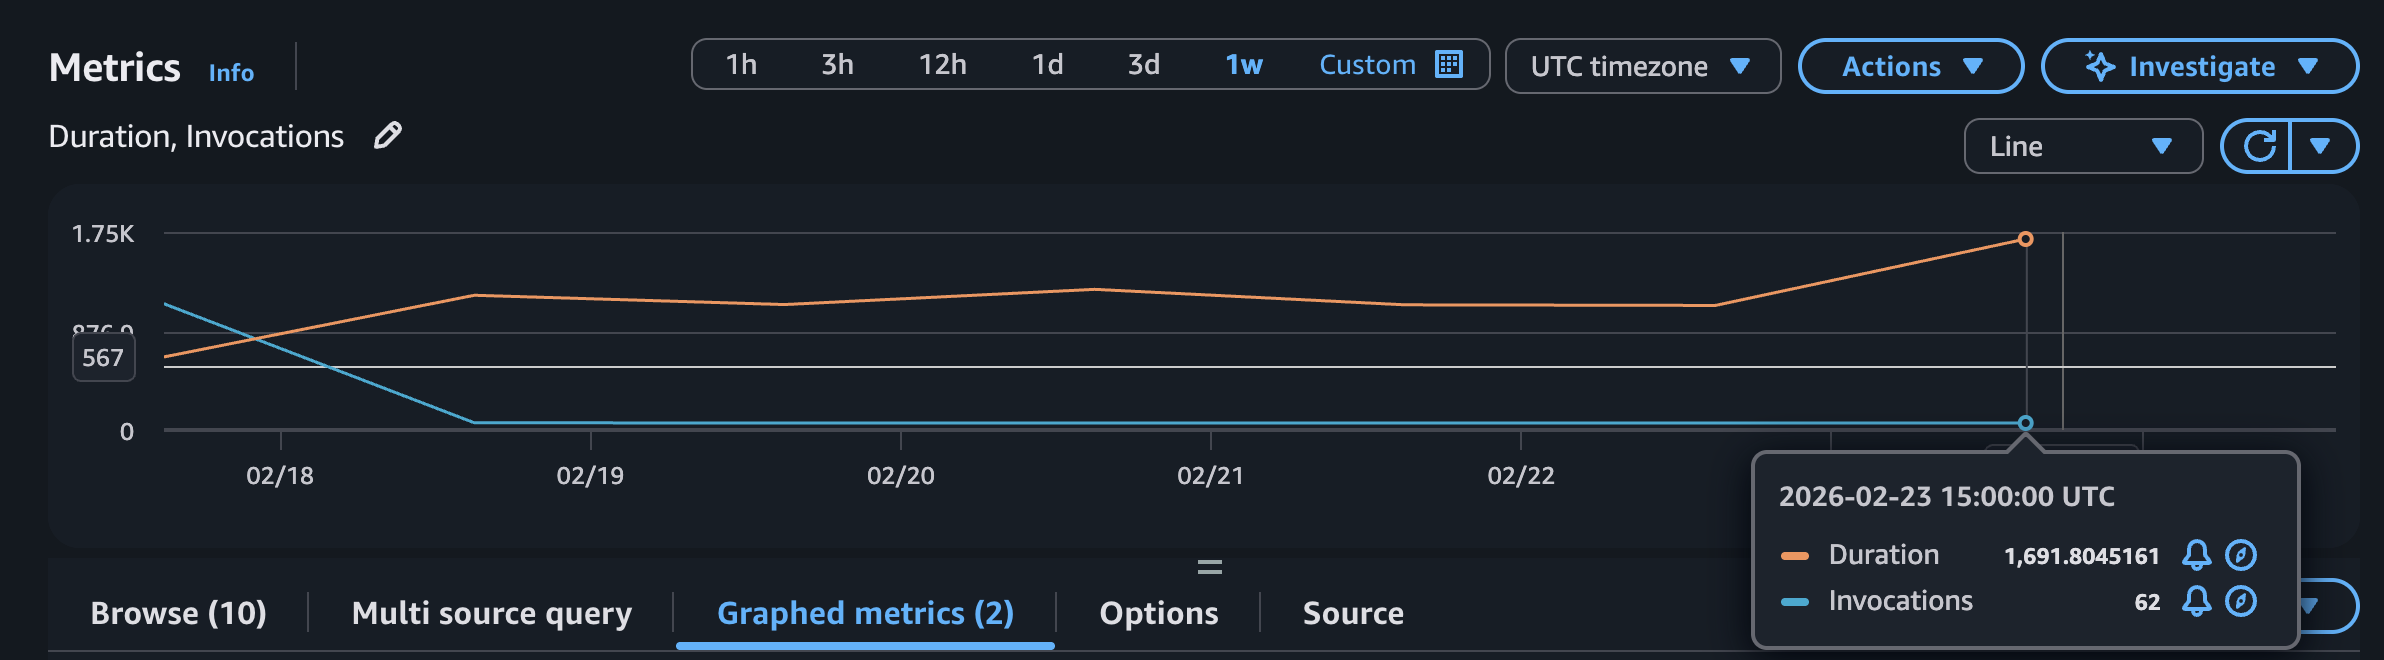
\includegraphics[width=1\textwidth]{images/invocations-durations-transformer.png}
\caption{Grafico CloudWatch illustrante il volume di invocazioni e la metrica Duration del livello Transformer.}
\label{fig:transformer-graphic}
\end{figure}

Come riportato nella Tabella \ref{tab:dimensionale-parquet}, la serializzazione finale in formato Apache Parquet con algoritmo di compressione Snappy produce una riduzione misurabile del footprint di archiviazione.

\begin{table}[htbp]
\centering
\caption{Confronto dimensionale empirico tra i payload estratti (Raw JSON/CSV) e i file ottimizzati (Clean Parquet).}
\label{tab:dimensionale-parquet}
\small
\begin{tabularx}{\textwidth}{lRR}
\toprule
\textbf{Tipologia di Report} & \textbf{Dimensione Raw} & \textbf{Dimensione Clean (Parquet)} \\
\midrule
get\_all\_line\_items & 654.6 MB & 1.6 MB \\
open\_header\_bidding & 161.2 MB & 45.7 MB \\
key\_value & 24.4 MB & 40.9 MB \\
kpis\_by\_hour & 3.7 MB & 2.0 MB \\
adrequest\_by\_hour & 1.4 MB & 921.3 KB \\
get\_all\_custom\_fields & 27.1 KB & 6.0 KB \\
\bottomrule
\end{tabularx}
\end{table}

Il fattore di compressione incide in misura maggiore sui documenti di grandi dimensioni, riducendo il file \texttt{get\_all\_line\_items} di un fattore superiore a 400. Eventuali incrementi dimensionali su file nell'ordine dei byte costituiscono un comportamento fisiologico imputabile alla dimensione minima dei metadati intrinseci richiesti dallo schema Parquet.

\subsection{Ottimizzazione dell'Interrogazione tramite Partition Pruning}
L'ultima fase del collaudo per la pipeline asincrona valuta l'impatto del partizionamento logico sui costi operativi e sulle latenze di Amazon Athena. L'indagine quantifica l'efficienza algoritmica della topologia a partizioni multiple, organizzata gerarchicamente per anno, mese e giorno. Il test esegue una serie di interrogazioni SQL sulla tabella non aggregata relativa alle impressioni pubblicitarie. La Tabella \ref{tab:athena-performance} sintetizza i risultati prestazionali estratti dal servizio cloud.

\begin{table}[htbp]
\centering
\caption{Confronto analitico delle prestazioni di scansione del motore distribuito Amazon Athena.}
\label{tab:athena-performance}
\small
\begin{tabularx}{\textwidth}{Xrr}
\toprule
\textbf{Modalità di Interrogazione} & \textbf{Tempo di Esecuzione} & \textbf{Dati Scansionati} \\
\midrule
Scansione Completa (Assenza di partizioni) & 15,37 secondi & 3,82 GB \\
Scansione Ottimizzata (Partition Pruning applicato) & 541 millisecondi & 3,90 MB \\
\bottomrule
\end{tabularx}
\end{table}

Il primo scenario di test definisce l'esecuzione di una query aggregata sull'intero storico dei dati. L'assenza di predicati temporali forza il motore distribuito a eseguire una scansione sequenziale completa dei file archiviati. Come illustrato nella Figura \ref{fig:athena-full-scan}, l'operazione comporta la lettura di $3,82$ GB di dati in $15,3$ secondi, impegnando le risorse in modo direttamente proporzionale alla dimensione totale del Data Lake.

\begin{figure}[htbp]
\centering
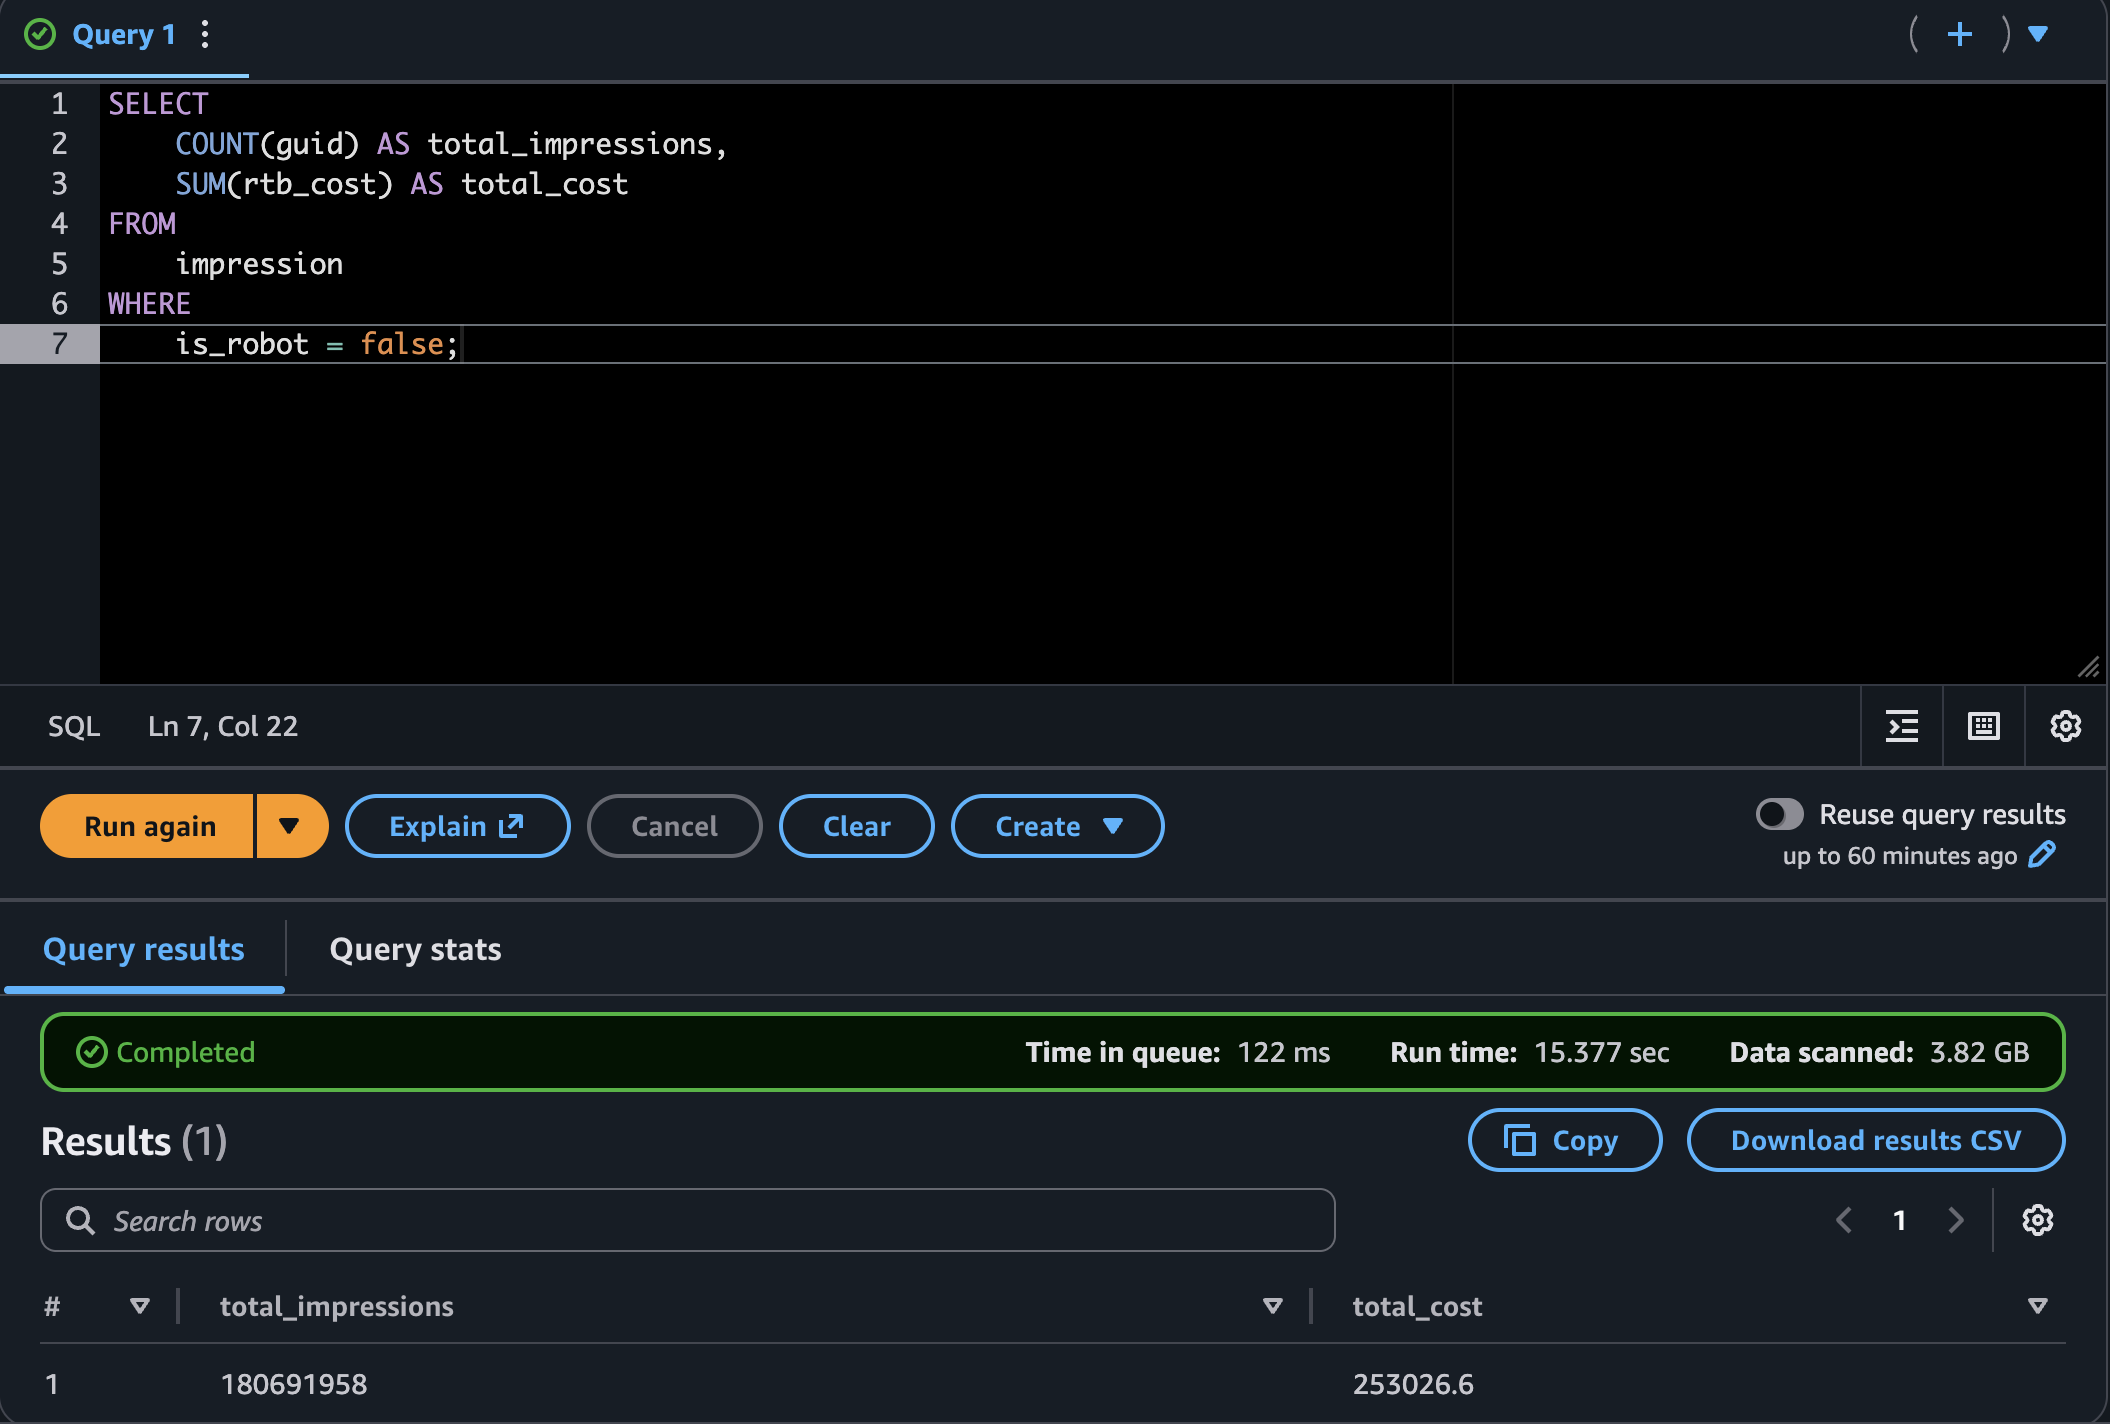
\includegraphics[width=\textwidth]{images/athena_full_scan.png}
\caption{Interfaccia di Amazon Athena: esecuzione di una query priva di partizionamento.}
\label{fig:athena-full-scan}
\end{figure}

Il secondo scenario applica il meccanismo di partition pruning, introducendo predicati temporali nella clausola \texttt{WHERE} per restringere il perimetro di ricerca a una singola giornata operativa. Il motore di Athena interroga il catalogo dati per escludere i prefissi non pertinenti prima di accedere allo storage. La Figura \ref{fig:athena-partition-pruning} riporta i risultati prestazionali di questa seconda esecuzione.

\begin{figure}[htbp]
\centering
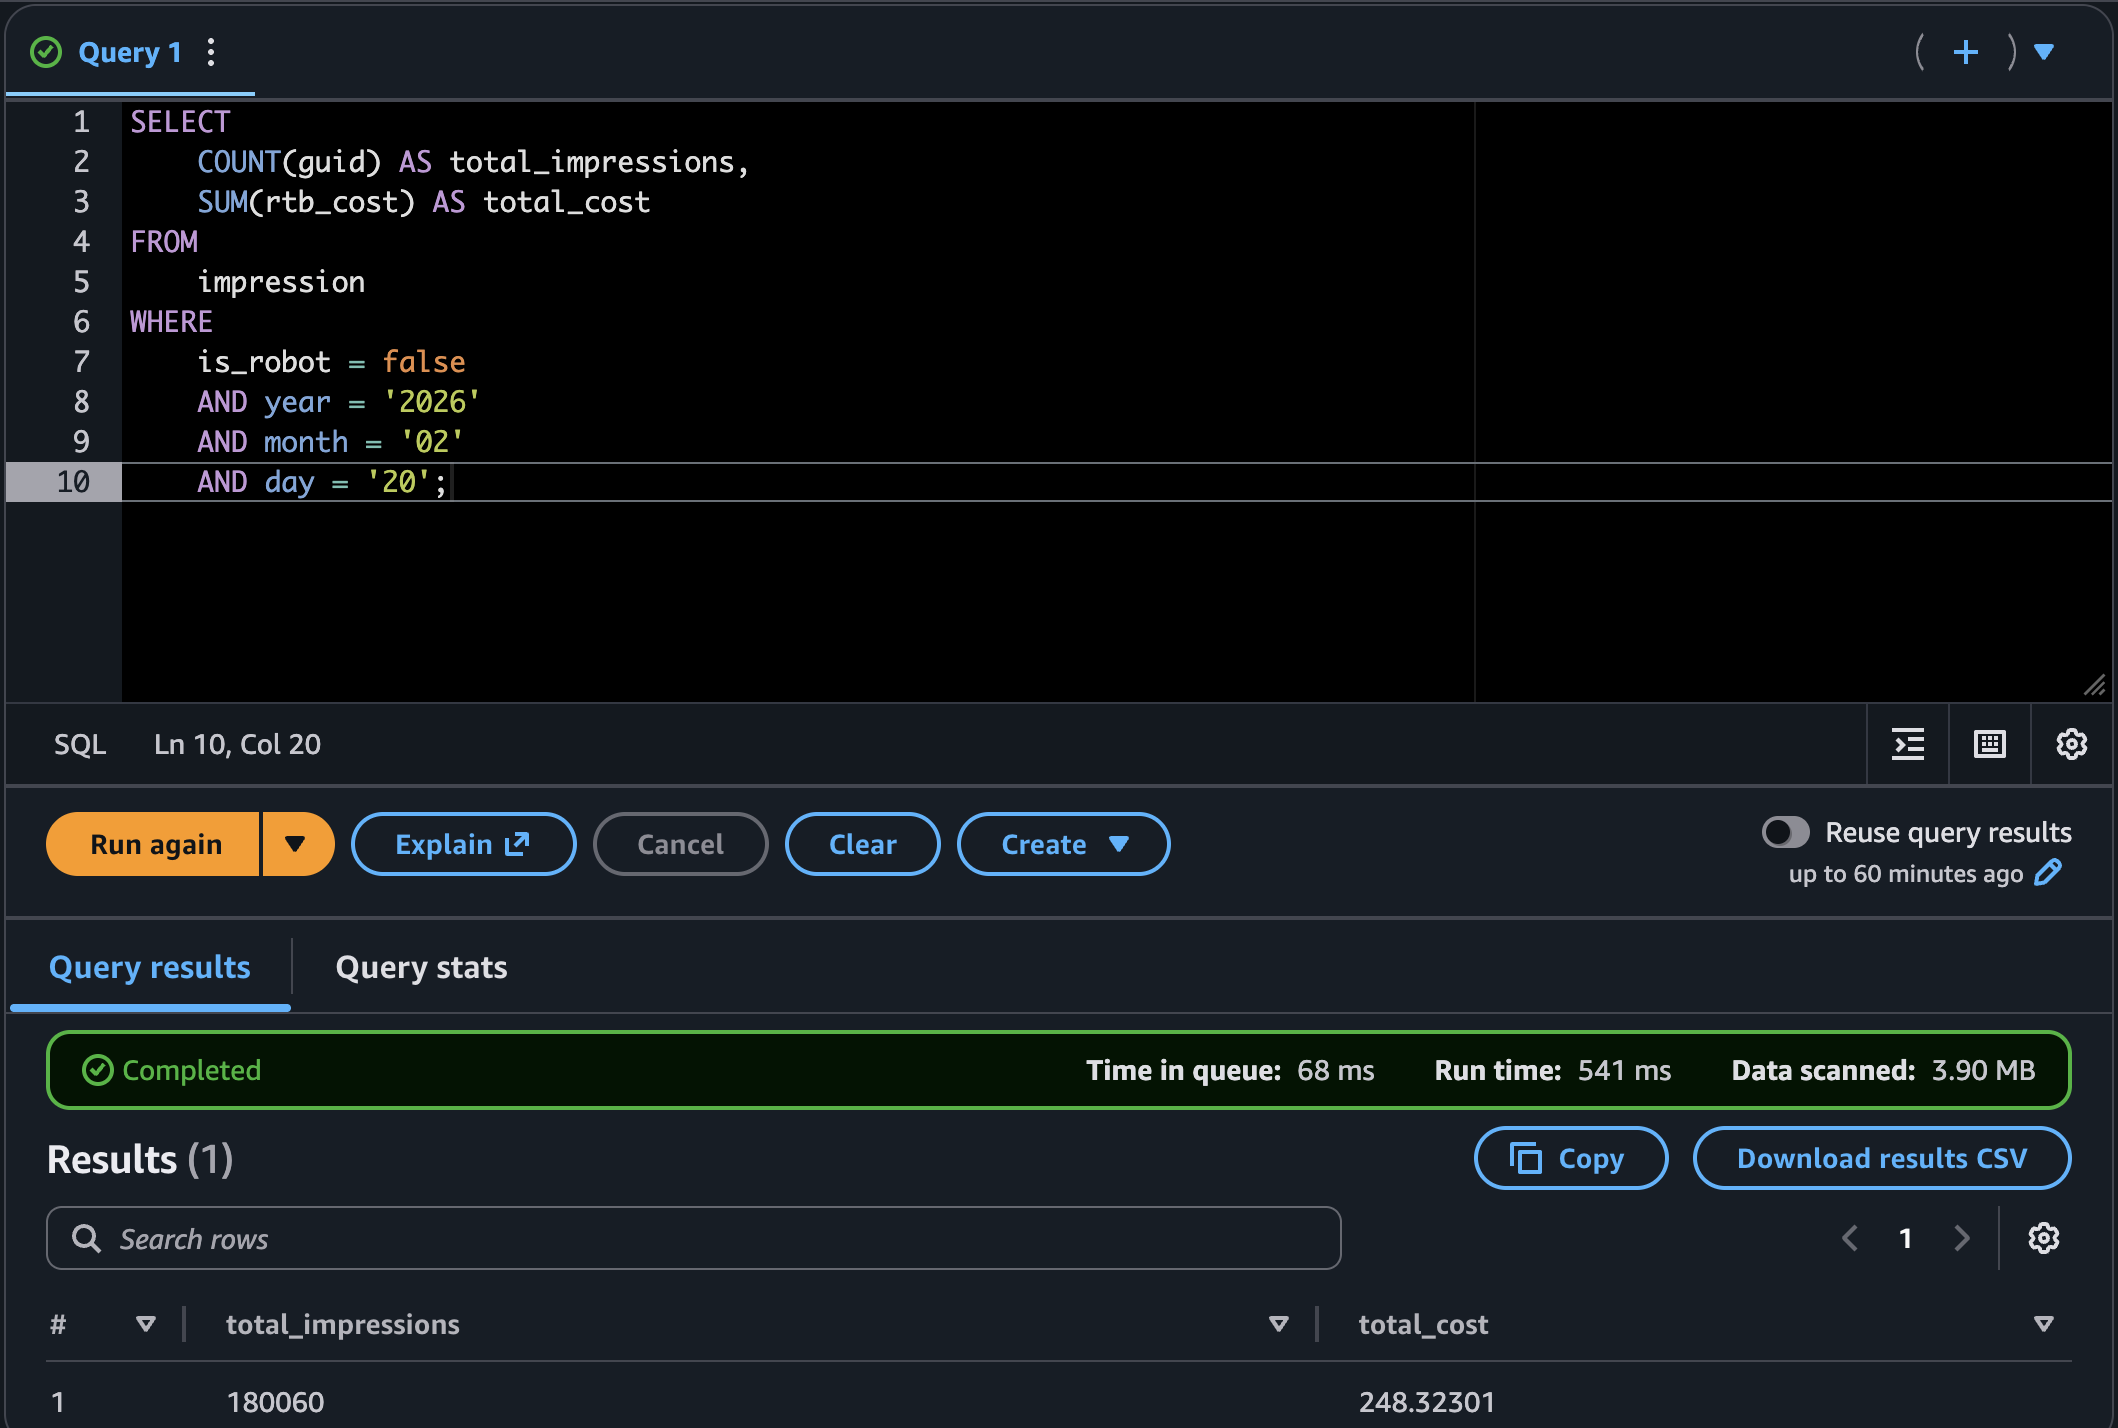
\includegraphics[width=\textwidth]{images/athena_optimized_scan.png}
\caption{Interfaccia di Amazon Athena: esecuzione di una query ottimizzata tramite partition pruning.}
\label{fig:athena-partition-pruning}
\end{figure}

Il partizionamento logico riduce il volume dei dati scansionati a $3,90$ MB e abbatte il tempo di elaborazione a $541$ millisecondi. L'abbattimento delle letture su disco dimostra che l'isolamento deterministico dei prefissi disaccoppia il tempo e il costo di interrogazione dalla mole totale dei dati immagazzinati nel sistema.

\section{Analisi quantitativa dei costi}
L'indagine economica valuta l'impatto del paradigma Serverless confrontando il modello a consumo con l'allocazione statica delle risorse, impiegando i parametri di fatturazione per la regione eu-west-1. L'analisi utilizza i dati volumetrici misurati nel primo caso di studio durante una settimana operativa. La quantificazione economica si struttura su due vettori di costo: il livello di archiviazione per le interrogazioni interattive e il livello computazionale per la trasformazione dei dati.

Il primo parametro esaminato riguarda il livello di interrogazione tramite Amazon Athena, il cui modello prevede un costo fisso di $\$5.00$ per terabyte scansionato. La sorgente dati genera 994 Megabyte di dati grezzi giornalieri, equivalenti a circa 30 Gigabyte mensili. In assenza di ottimizzazioni, una singola query sulla giornata imporrebbe la lettura dell'intero archivio, generando un addebito di $\$0.14$. Il processo ETL converte i file in formato Parquet riducendo l'impronta a 107 Megabyte giornalieri, e il partizionamento logico istruisce il motore a leggere unicamente questa frazione. La convergenza di queste tecniche porta il costo della singola operazione a $\$0.0005$, confermando la sostenibilità finanziaria del sistema analitico.

Il secondo parametro economico concerne l'elaborazione computazionale. La funzione AWS Lambda di estrazione esegue 4079 invocazioni settimanali (50244 secondi di calcolo), mentre la trasformazione registra 1498 invocazioni (1215 secondi). Entrambe richiedono 6 Gigabyte di memoria. Proiettando le metriche su base mensile, l'infrastruttura consuma circa $1.32$ milioni di Gigabyte-secondo, traducendosi in una spesa di $\$17.65$ mensili sull'architettura ARM. Un'architettura tradizionale basata su un'istanza Amazon EC2 \cite{EC2} di classe c6g.xlarge (4 vCPU, 8 GB RAM) imporrebbe un costo fisso di $\$103.95$. Il modello basato su eventi riduce i costi di elaborazione dell'$83\%$, eliminando il dispendio economico intrinseco ai periodi di inattività.

\section{Caso di Studio II: Servizio Backend Sincrono}
Il secondo caso di studio valuta l'architettura a fronte di carichi operativi sincroni. Il perimetro di analisi coinvolge un'API interna sviluppata tramite il framework FastAPI ed esposta via API Gateway, concepita per la registrazione e il recupero dei metadati relativi a presentazioni multimediali. L'implementazione applica i paradigmi di astrazione precedentemente descritti per misurare le latenze di un'infrastruttura di backend interamente gestita dal cloud provider.

\subsection{Modello Dati ad Alta Efficienza}
La memorizzazione dello stato sfrutta il database NoSQL Amazon DynamoDB. La progettazione adotta il paradigma Single Table Design, modellato tramite la libreria PynamoDB. L'entità definisce una chiave di partizione primaria per l'accesso puntuale a complessità costante. Per supportare le interrogazioni sulle collezioni, la struttura implementa un Global Secondary Index (GSI) con chiave di partizione statica e chiave di ordinamento cronologica, come mostrato nel Listato \ref{lst:demoland-pynamo}.

\begin{lstlisting}[language=Python, caption={Modellazione Object-Relational Mapping (ORM) su DynamoDB.}, label={lst:demoland-pynamo}]
from pynamodb.models import Model
from pynamodb.attributes import UnicodeAttribute, BooleanAttribute
from pynamodb.indexes import GlobalSecondaryIndex, AllProjection
import os

class CreationDateIndex(GlobalSecondaryIndex):
    """
    This class represents a GSI for querying previews by creation_date.
    """
    class Meta:
        index_name = 'creation-date-index'
        projection = AllProjection()
    
    # This attribute will be the partition key for the GSI
    entity_type = UnicodeAttribute(hash_key=True)
    creation_date = UnicodeAttribute(range_key=True)

class Preview(Model):
    class Meta:
        table_name = os.environ.get("DYNAMODB_TABLE")
        region = os.getenv("AWS_DEFAULT_REGION")
    
    # GSI for sorting by creation_date
    creation_date_index = CreationDateIndex()

    # Primary key
    slug = UnicodeAttribute(hash_key=True)
    SLUG_MAX_ATTEMPTS = 10

    # GSI partition key - a static value to query all previews
    entity_type = UnicodeAttribute(default="PREVIEW")

    # Client and campaign information
    customer = UnicodeAttribute()
    normalized_customer = UnicodeAttribute()
    campaign = UnicodeAttribute()
    normalized_campaign = UnicodeAttribute()

    # Categorization fields
    vertical = UnicodeAttribute()
    format = UnicodeAttribute()
    type = UnicodeAttribute()

    # Technical fields
    webpage = UnicodeAttribute()
    script = UnicodeAttribute()

    # Configuration flags
    confidential = BooleanAttribute(default=False)
    live = BooleanAttribute(default=False)
    device = UnicodeAttribute(default="Mobile")

    # Location and language
    delivery_country = UnicodeAttribute(default="Italy")
    language = UnicodeAttribute(default="Italian")
    country = UnicodeAttribute(default="Simulated Entity")

    # Creation date
    creation_date = UnicodeAttribute(null=True)
\end{lstlisting}

Come evidenziato nella Tabella \ref{tab:dynamodb-capacity} e nella Figura \ref{fig:dynamodb-capacity}, la standardizzazione degli accessi limita il consumo delle unità di capacità di lettura e scrittura.

\begin{table}[htbp]
\centering
\caption{Medie di consumo orario delle unità di capacità sul livello DynamoDB.}
\label{tab:dynamodb-capacity}
\begin{tabular}{lr}
\toprule
\textbf{Metrica di Capacità (Media Oraria)} & \textbf{Valore Rilevato} \\
\midrule
Consumed Read Capacity Units (RCU) & 0.005 \\
Consumed Write Capacity Units (WCU) & 0.062 \\
\bottomrule
\end{tabular}
\end{table}

\begin{figure}[htbp]
\centering
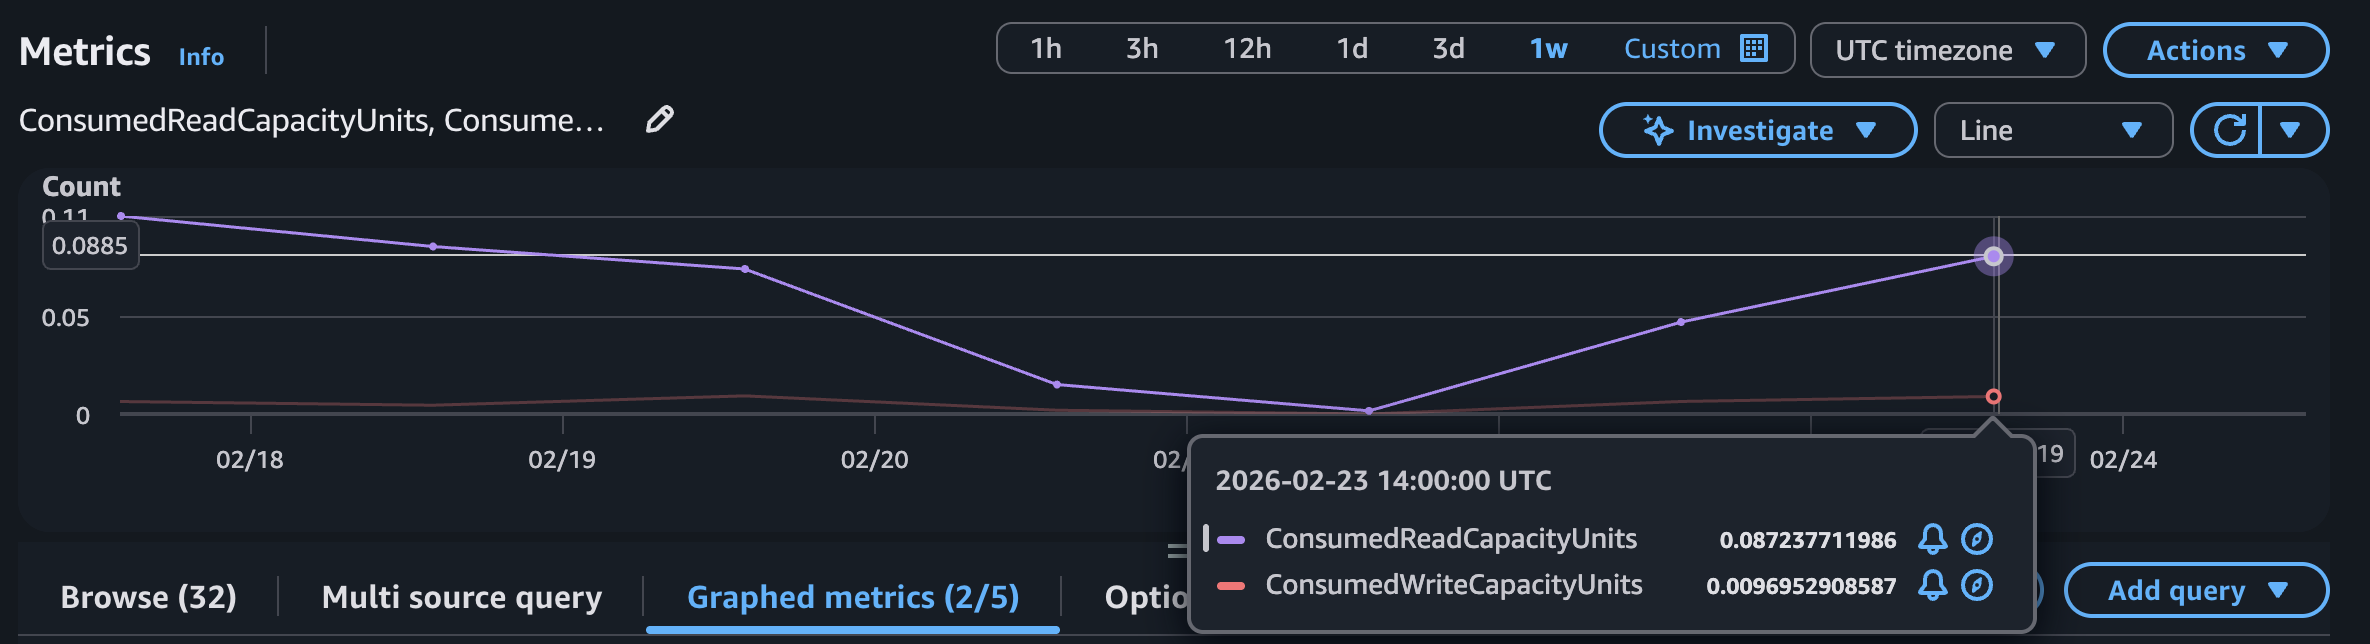
\includegraphics[width=1\textwidth]{images/capacity-dynamo.png}
\caption{Grafico CloudWatch illustrante l'andamento temporale della capacity di DynamoDB per il servizio.}
\label{fig:dynamodb-capacity}
\end{figure}

Il contenimento delle capacità consumate garantisce la scalabilità del catalogo limitando l'impatto economico associato alle operazioni concorrenti.

\subsection{Distribuzione Statistica della Latenza e Cold Start}
L'esecuzione del framework web all'interno dell'ambiente di calcolo effimero necessita dell'adattatore Mangum. La telemetria calcola i percentili statistici dei tempi di integrazione esposti all'utente per misurare l'incidenza di questo strato di traduzione. I dati aggregati sono presentati nella Tabella \ref{tab:percentili-latenza} e graficati nella Figura \ref{fig:api-gateway-latency}.

\begin{table}[htbp]
\centering
\caption{Distribuzione statistica dei percentili di latenza di integrazione (in millisecondi).}
\label{tab:percentili-latenza}
\begin{tabular}{lr}
\toprule
\textbf{Percentile Statistico} & \textbf{Latenza Rilevata (ms)} \\
\midrule
50° Percentile ($p50$ - Mediana) & 19.5 ms \\
90° Percentile ($p90$) & 708.5 ms \\
99° Percentile ($p99$) & 1751.9 ms \\
\bottomrule
\end{tabular}
\end{table}

\begin{figure}[htbp]
\centering
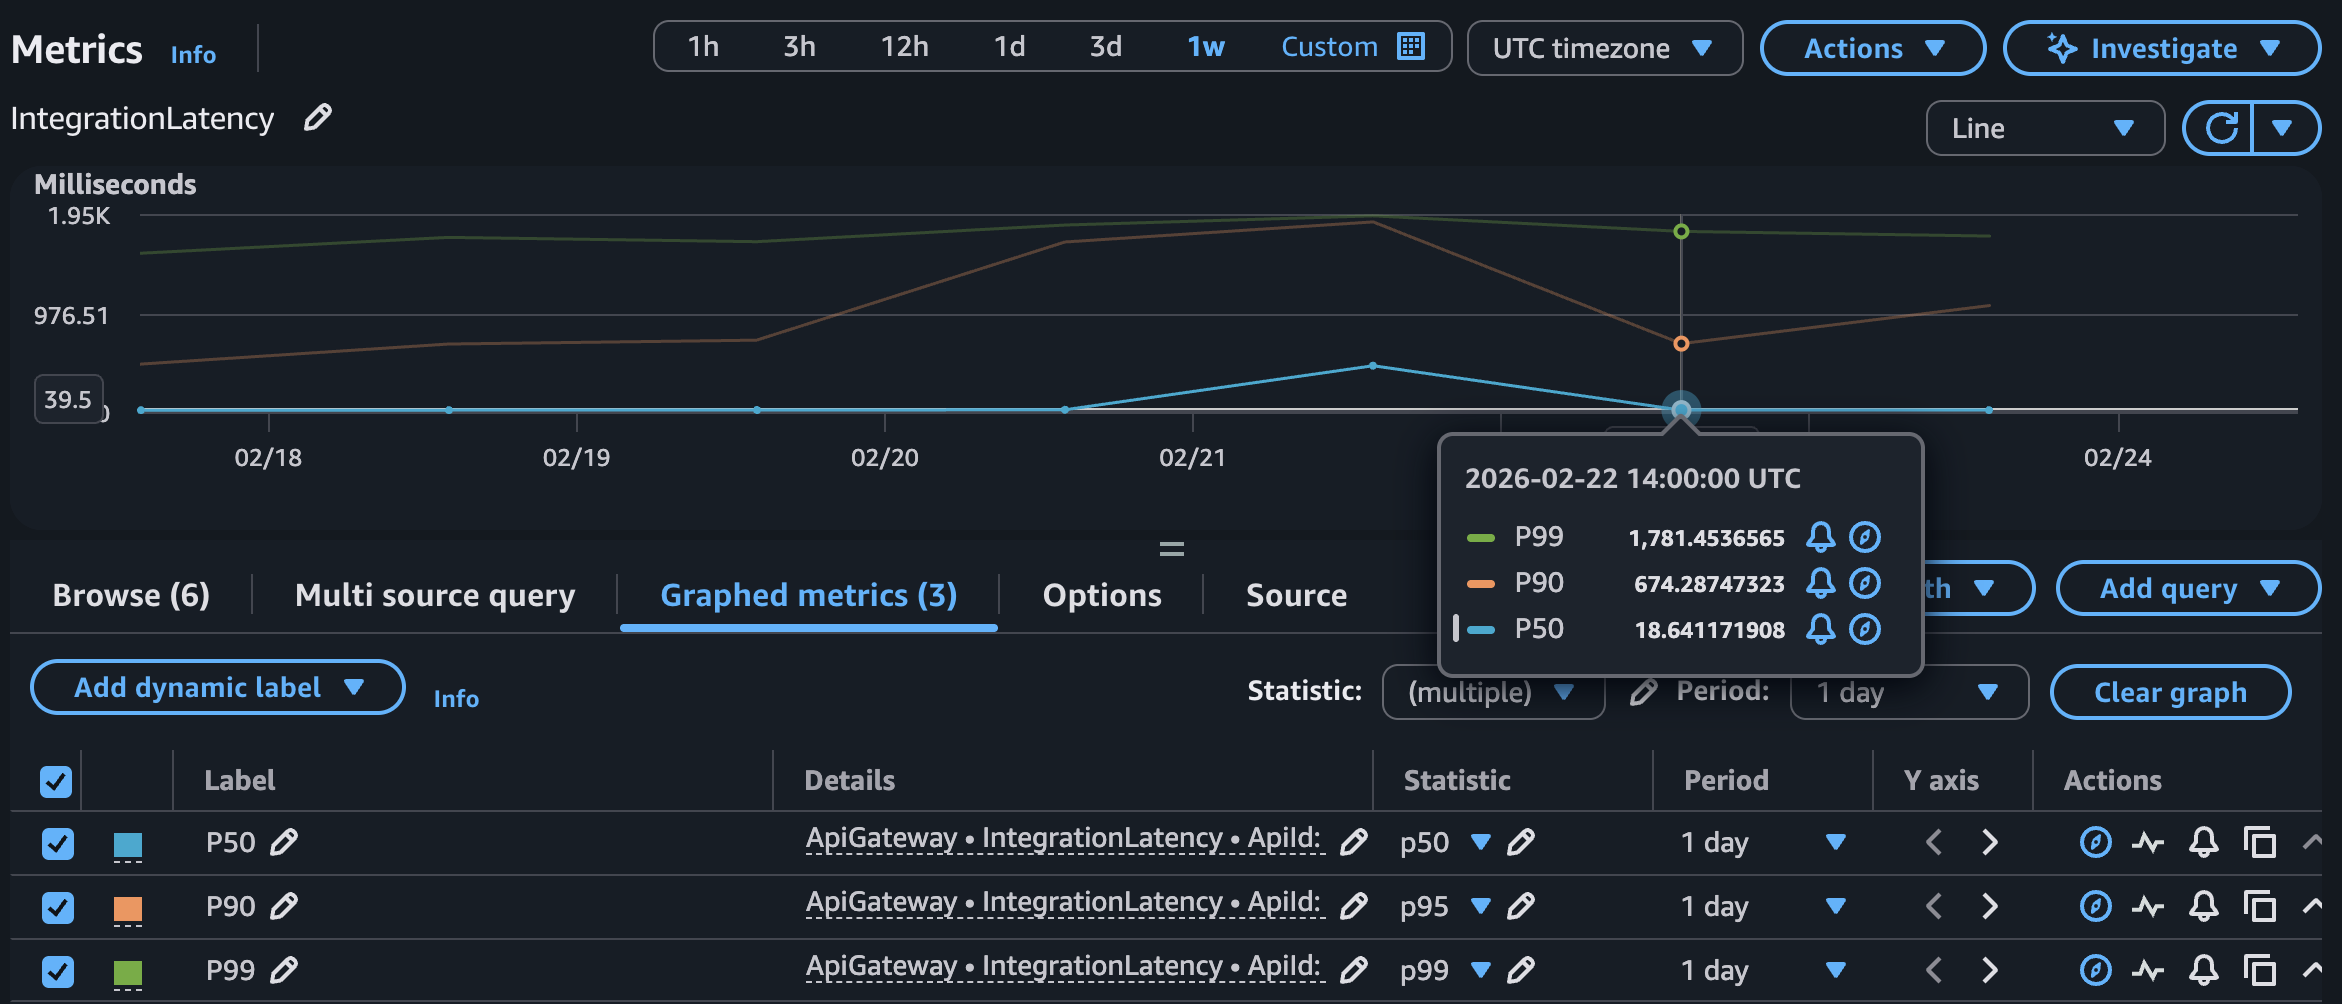
\includegraphics[width=1\textwidth]{images/percentili-api-gateway.png}
\caption{Grafico CloudWatch illustrante l'andamento temporale dei percentili di latenza p50, p90 e p99.}
\label{fig:api-gateway-latency}
\end{figure}

Il tempo di risposta mediano ($p50$) attesta che l'adattatore non introduce sovraccarichi penalizzanti nei container già in esecuzione. L'analisi dei percentili di coda ($p90$ e $p99$) quantifica empiricamente il peso delle latenze di inizializzazione dell'ambiente (Cold Start), le quali portano i tempi di risposta oltre la soglia dei 1700 millisecondi. La varianza rientra nei limiti di tolleranza per i requisiti non funzionali del sistema in analisi.

\section{Valutazione dell'Automazione Infrastrutturale (Service-Forge)}
L'ultima fase dell'analisi quantifica l'impatto architetturale derivante dall'adozione del framework interno dedicato allo scaffolding. Il sistema standardizza il provisioning di nuovi microservizi astraendo la complessità dichiarativa dell'Infrastructure as Code (IaC). La valutazione esamina tre distinte metodologie di generazione, misurando per ciascun approccio il carico cognitivo richiesto all'operatore, l'esposizione al rischio operativo e i tempi di esecuzione. La Tabella \ref{tab:scaffolding-comparison} sintetizza il confronto.

\begin{table}[htbp]
\centering
\caption{Confronto analitico tra le metodologie di generazione infrastrutturale (Scaffolding).}
\label{tab:scaffolding-comparison}
\small
\begin{tabularx}{\textwidth}{lXXX}
\toprule
\textbf{Metrica di Valutazione} & \textbf{Scaffolding Manuale} & \textbf{Scaffolding CLI (Typer)} & \textbf{Scaffolding MCP (FastMCP)} \\
\midrule
Tempo di approvvigionamento & Misurabile in ore & Misurabile in minuti & Limitato a pochi secondi \\
Deriva di Configurazione & Alta esposizione & Assente (uso di Jinja2) & Assente (motore AI confinato) \\
Carico Cognitivo Operatore & Livello elevato & Livello moderato & Livello minimo \\
Aderenza al Least Privilege & Dipendente dall'operatore & Garantita dal template & Rigorosamente applicata \\
\bottomrule
\end{tabularx}
\end{table}

Le metodologie analizzate seguono tre approcci procedurali. La prima metodologia prevede la configurazione integralmente manuale degli artefatti. L'operatore definisce i moduli Terraform, le configurazioni Docker e i flussi CI/CD scrivendo direttamente il codice sorgente. Questo approccio impone un livello di attenzione elevato e richiede all'operatore una conoscenza pregressa e trasversale dello stack tecnologico. L'esecuzione manuale espone il sistema a un'alta probabilità di deriva di configurazione. I tempi di approvvigionamento per un singolo microservizio risultano quantificabili nell'ordine delle ore.

La seconda metodologia impiega un'interfaccia a riga di comando (CLI) in grado di elaborare template deterministici basati sul motore Jinja2. Il sistema inietta i parametri forniti dall'utente all'interno di strutture predefinite. L'astrazione riduce i tempi operativi a pochi minuti ed elimina il rischio di deriva di configurazione, poiché i template impongono l'applicazione rigorosa dei vincoli di sicurezza. Lo strumento mantiene un vincolo operativo: l'operatore deve conoscere a priori la nomenclatura esatta e la tipologia dei parametri infrastrutturali richiesti.

La terza metodologia introduce il Model Context Protocol (MCP) per delegare l'interazione iniziale a un agente basato su Large Language Models (LLM). L'architettura confina la comunicazione non deterministica alla sola interfaccia testuale dell'ambiente di sviluppo integrato. L'agente estrae le specifiche dal linguaggio naturale e invoca la logica di generazione deterministica sottostante tramite chiamate strutturate. Questa interazione riduce il tempo di generazione a pochi secondi e minimizza il carico cognitivo.

L'impiego dei modelli linguistici introduce problematiche intrinseche di affidabilità, legate alla natura probabilistica della generazione del testo. L'analisi del comportamento dell'agente conversazionale evidenzia scenari in cui il modello interrompe prematuramente la negoziazione dei parametri, tentando di avviare il processo di scaffolding senza fornire identificativi obbligatori. Il server FastMCP previene questa inesattezza applicando una validazione statica dei tipi sui payload JSON in ingresso. Il motore intercetta le richieste malformate, blocca preventivamente l'esecuzione e restituisce l'errore semantico all'ambiente di sviluppo, forzando l'LLM a reiterare la richiesta verso l'utente umano.